\begin{figure}
\section{Ontology Service}
Ontology Service is a facility to offer users the access ability to 
an ontology resource. Click on the OntoService link from the menu of 
each page, you will reach the ontology repository list page, as shown 
below.
\newline
\newline
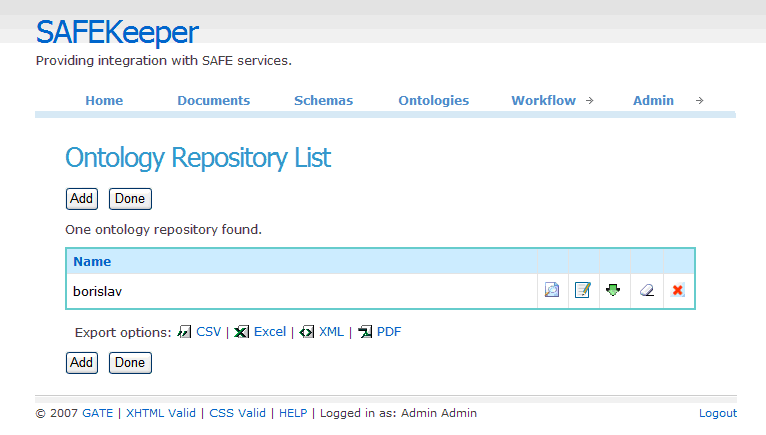
\includegraphics[scale=0.4]{ontorepolist}
\caption{Ontology Repository List}
\label{fig:ontorepolist}
\end{figure}

\begin{figure}
To add a new ontology repository, simply click on the Add button on 
the above page and you should reach the following page where you can 
specify the ontology name and its URL.
\newline
\newline
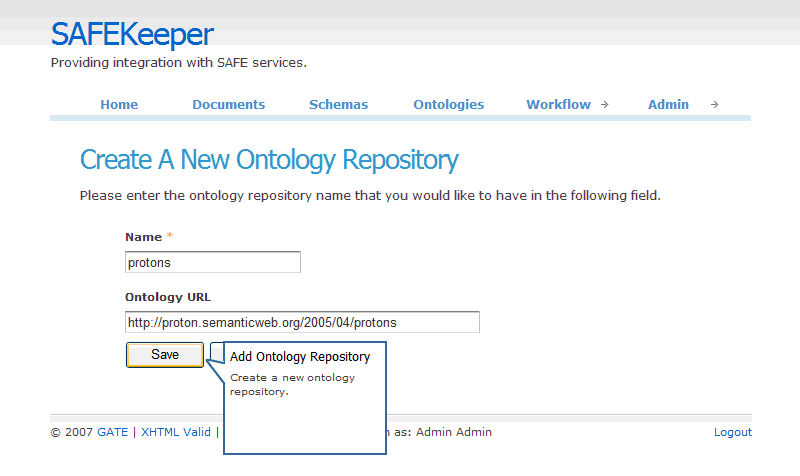
\includegraphics[scale=0.4]{addontorepo}
\caption{Add Ontology Repository}
\label{fig:addontorepo}
\end{figure}

\begin{figure}
After clicking on the Save button from the above page, you should see
the prompt message and the ontology repository you populated from the
remote URL just now.
\newline
\newline
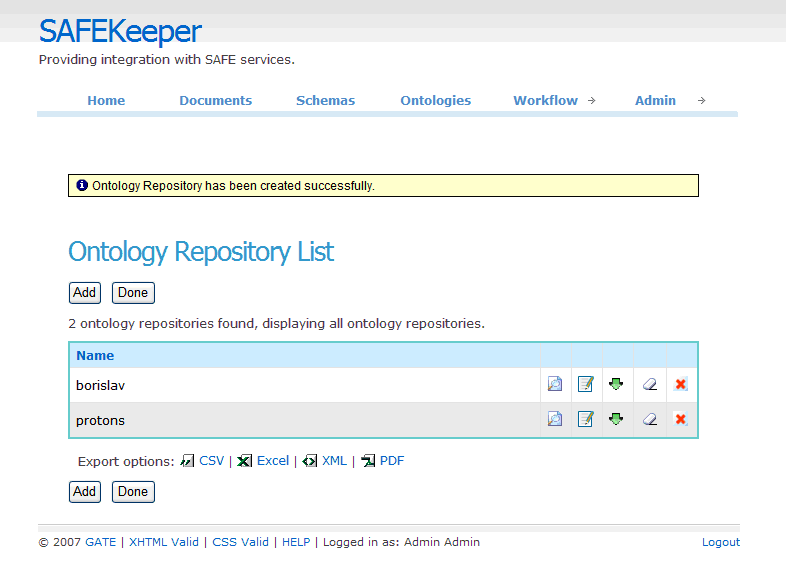
\includegraphics[scale=0.4]{ontorepoadded}
\caption{Ontology Repository Added}
\label{fig:ontorepoadded}
\end{figure}

\begin{figure}
To view the content of the ontology repository, click on the view icon
in the 2nd column of table above. Then you should reach the following 
page, where you can also download the ontology to your disk.
\newline
\newline
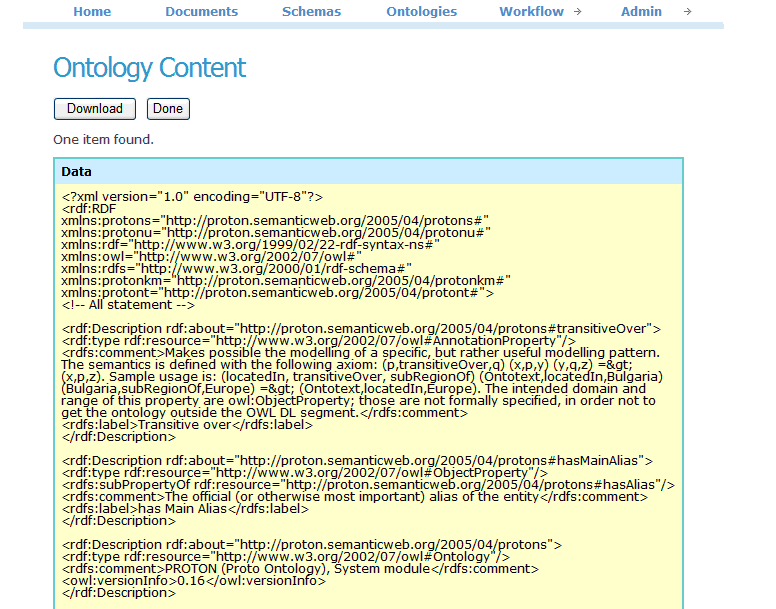
\includegraphics[scale=0.4]{ontorepoview}
\caption{View Ontology Repository}
\label{fig:ontorepoview}
\end{figure}

\begin{figure}
To update an ontology repository, you have two choices: either merge 
the existing ontology with a new one or replace it with the new one, 
which is shown as below.
\newline
\newline
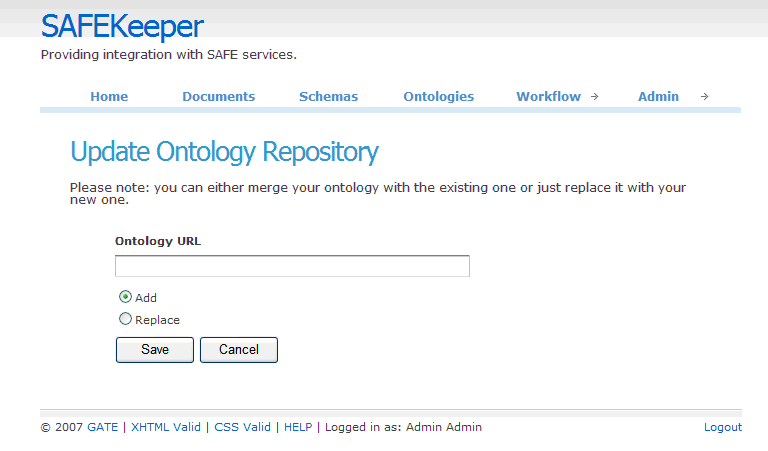
\includegraphics[scale=0.4]{updateontorepo}
\caption{Update Ontology Repository}
\label{fig:updateontorepo}

To empty an ontology repository or delete it, simply click on the 
relevant icons on the ontology repository list page.
\end{figure}

\newpage
\clearpage
